% homework/hw10/hw10.tex
% Year 7 - Homework Packet 10: Faster in January.
%
% Two parts, at the teacher's request (22 October 2026): "bake the decimals
% into the science, but add more math review of unit 4".
%   Part 1  Sections A-C. Unit 4 again, all of it, with new numbers: compare,
%           add and subtract (4.1-4.2), multiply and divide including by a
%           2-digit number (4.3-4.4 and the review), the quick ways (4.5),
%           money, and the words that choose the operation.
%   Part 2  Sections D-F. Science 3.2 (formation of the Solar System), 3.3
%           (movement in space) and Models Part 1 (the football Sun). D and E
%           are the science in words; F does it in decimals.
% No Extra sheet goes with this packet: the Science Models challenge
% (homework/caffeine) is the extra this week.
%
% Section F is why this packet exists. F3 is 3.3's exit question -- the Earth
% is closer to the Sun in January than in July, so when does it move faster?
% -- answered with the real numbers: 30.3 km/s in January, 29.3 km/s in July.
% The difference is 1.0 km/s, the MEAN is 29.8 km/s, and 29.8 rounded to the
% nearest whole number is 30: the Earth's speed in the book's table. So the
% book's 30 is a mean, rounded, and the decimals say so.
% F1 is the other trap worth the section: "how much faster" (subtract) and
% "how many times as fast" (divide) on the same pairs of planets, side by side.
%
% Nothing untaught:
%   * Planet speeds are the 3.3 deck's (the book's Activity table, whole
%     km/s): Mercury 48, Venus 35, Earth 30, Mars 24, Jupiter 13, Saturn 10,
%     Uranus 7, Neptune 5. Every "times as fast" in F1 comes out exact.
%   * The Earth's January and July figures are NASA's, to 1 d.p.: 147.1 and
%     152.1 million km; 30.29 and 29.29 km/s. The rule they test is 3.3's
%     write note (speed decreases as distance increases).
%   * The football model is the Models deck's ScaleShrink widget (sizes.jsx):
%     Sun 22 cm, Earth 2 mm and 24 m away, Moon 0.5 mm, Jupiter 2.3 cm,
%     Neptune 7.8 mm (shown rounded to 8 mm on the slide).
%   * The 3.2 facts are the deck's: one spinning cloud; same direction, same
%     plane; Venus spins the opposite way; Uranus spins on its side; HL Tauri;
%     most moons orbit the same way; the Sun has 99.8% of the mass.
%   * Nothing is decimal x decimal. Every division by a 2-digit number has a
%     times table to write.
%   * No number is lifted from the workbook, from HW 9 or EX 9, or from the
%     decks' practice panels.
%
% House style is shared: see homework/hw-style.tex. Method: the new-homework
% skill. Source is pure ASCII on purpose.
%
% Build:  pwsh .claude/skills/new-homework/scripts/build-hw.ps1 hw10 -French

\documentclass[12pt,a4paper]{article}

% -- Answer key switch -------------------------------------------------------
\newif\ifkey
\ifdefined\TEACHER\keytrue\else
  \keyfalse        % \keyfalse = student copy   |   \keytrue = teacher copy
\fi

% -- Language switch ---------------------------------------------------------
% The French copy (hw10-fr.pdf) is this file built with \FRENCH defined. See
% hw09/README.md for the scheme.
\newif\iffr
\ifdefined\FRENCH\frtrue\fi

% -- House style -------------------------------------------------------------
% homework/hw-style.tex
% Shared house style for every Year 7 homework packet. \input this from the
% packet file, right after \documentclass and the answer-key switch.
%
% Do not fork this file per packet. If a packet needs a different look, the
% question is whether every packet should have it.
%
% The choices here are deliberate and were arrived at by printing and looking:
%   * No solid dark banners. Every header is a light tint with a coloured spine
%     on the left, so colour reads clearly without flooding a school printer.
%   * No marks and no mark totals. These are practice, not exam papers.
%   * Lato at 12pt with open leading, plus mathastext so inline maths is Lato
%     too. Without mathastext every "-6 + 4" is Computer Modern serif and the
%     sheet looks half-typeset.
%   * Writing lines are spaced for Year 7 handwriting, not adult margin notes.
%   * Pages fill. \needspace is redefined below so a heading no longer drags
%     the page break up to itself, and every heading is glued to the box under
%     it. Packets built before 2026-09-30 were laid out under the old rules and
%     will reflow if rebuilt -- re-read every page if you rebuild one.
%
% Provides: \wlines \blank \tickbox \sep \qmk-free marks (none) \hwsection
% \qhead \expr, the workspace box, and the remember / wordhelp / activity /
% yourturn coloured boxes. Palette matches the lesson decks exactly.

% -- Packages ----------------------------------------------------------------
\usepackage[T1]{fontenc}
\usepackage[utf8]{inputenc}
\usepackage[default]{lato}
\usepackage[a4paper,top=1.7cm,bottom=1.7cm,left=2.0cm,right=2.0cm,headheight=15pt]{geometry}
\usepackage{amsmath,amssymb}
\usepackage{xcolor}
\usepackage[most]{tcolorbox}
\usepackage{enumitem}
\usepackage{tikz}
\usetikzlibrary{arrows.meta}
\usepackage{array}
\usepackage{tabularx}
\usepackage{fancyhdr}
\usepackage{multicol}
\usepackage{needspace}
\usepackage{graphicx}

% Make maths use Lato too. Without this, every "-6 + 4" on the page is set in
% Computer Modern serif and the sheet looks half-typeset. Must come last.
\usepackage[italic]{mathastext}

% -- \needspace, without the hole it used to leave ----------------------------
% needspace.sty writes "\vskip 0pt plus X \penalty-100" in front of every
% heading. A page that ends anywhere else is underfull with no stretch, so TeX
% scores it b=10000; a page that ends AT a heading gets that X of stretch and a
% finite badness, and wins. So any heading in roughly the bottom half of a page
% claimed the break, and the question under it moved over whole, leaving a hole
% the size of the question. \tracingpages showed it exactly (b=4531 at the
% heading, b=10000 at every later break) while building homework/q1rev, and it
% is where the half-empty pages in HW 1-8 came from.
% This keeps only the \penalty9999, which still refuses to put a heading in the
% last X of a page. Keeping a heading WITH the box under it is \nobreak's job
% now -- see \hwsection and \qhead below.
\makeatletter
\renewcommand{\needspace}[1]{\begingroup\setlength{\dimen@}{#1}%
  \vskip\dimen@\penalty9999\vskip-\dimen@\endgroup}
\makeatother

\linespread{1.06}\selectfont

% -- The Learner's Book palette (same hex values as the lesson decks) ---------
\definecolor{cbteal}{HTML}{0087A8}
\definecolor{cbpurple}{HTML}{5C2483}
\definecolor{cborange}{HTML}{C25E12}
\definecolor{cbgreen}{HTML}{4A8B23}
\definecolor{cbred}{HTML}{C8102E}
\definecolor{cbblue}{HTML}{1A5FA8}
\definecolor{rulegray}{HTML}{9AA5AD}

% -- Answer lines and blanks -------------------------------------------------
% \wlines{n} draws n ruled writing lines, spaced wide enough for Year 7
% handwriting rather than for an adult with a fine pen.
\makeatletter
\newcommand{\wlines}[1]{%
  \par\vspace{0.75em}%
  \@tempcnta=0\relax
  \@whilenum\@tempcnta<#1\do{%
    \hbox to \linewidth{\color{rulegray}\leaders\hrule height 0.5pt\hfill}%
    \vspace{1.5em}%
    \advance\@tempcnta by 1\relax}%
  \par\vspace{-0.8em}%
}
\makeatother

% \blank[width] is an inline gap to write a short answer in.
\newcommand{\blank}[1][2.6cm]{\underline{\hspace{#1}}}

% A boxed space for showing working.
\newtcolorbox{workspace}[1][3.4cm]{%
  colback=white, colframe=rulegray, boxrule=0.5pt, arc=5pt,
  height=#1, left=6pt, right=6pt, top=4pt, bottom=4pt,
  before skip=9pt, after skip=11pt}

% An empty tick box.
\newcommand{\tickbox}{\fbox{\rule{0pt}{1.15em}\rule{1.15em}{0pt}}}

% A middot separator.
\newcommand{\sep}{\,\textperiodcentered\,}

% -- Section and question headings -------------------------------------------
% Light tint plus a fat coloured spine on the left. No solid dark banner: the
% colour reads clearly but barely costs the printer anything.
% needspace keeps a heading out of the last few lines of a page. The \nobreak
% after it keeps it with whatever comes next: a remember or word-help box that
% does not fit takes its heading over with it, instead of leaving the heading
% alone at the foot of the page. (The old needspace did that by accident, and
% left a hole every time; see above.)
\newcommand{\hwsection}[2][cbteal]{%
  \needspace{8\baselineskip}%
  \par\vspace{13pt}%
  \noindent
  \begin{tcolorbox}[enhanced, nobeforeafter, width=\textwidth,
      colback=#1!7, colframe=#1!7, arc=5pt,
      borderline west={5pt}{0pt}{#1},
      left=14pt, right=10pt, top=7pt, bottom=7pt]
    {\large\bfseries\color{#1}#2}
  \end{tcolorbox}%
  \par\nobreak\vspace{9pt}}

% \qhead[colour]{A2}{Moving along the line} -- a question heading.
\newcommand{\qhead}[3][cbteal]{%
  \needspace{6\baselineskip}%
  \par\vspace{11pt}%
  \noindent{\large\bfseries\color{#1}#2}\quad{\large\bfseries #3}\par\nobreak\vspace{4pt}}

% -- Coloured boxes ----------------------------------------------------------
% Shared look: rounded, light fill, coloured rule, coloured title text on a
% pale title strip rather than a dark one.
% NOT breakable. A breakable box that cannot fit its first lines forces its own
% page break, and \nobreak cannot stop a forced break -- so the heading above
% it was left alone at the foot of the page (tested: it happens with \nobreak
% in place). Unbreakable, the page builder moves heading and box together.
% These boxes are a few lines each; none needs to split.
\tcbset{hwbox/.style={
  enhanced, arc=6pt, boxrule=1pt,
  left=11pt, right=11pt, top=8pt, bottom=8pt,
  fonttitle=\bfseries, attach boxed title to top left={xshift=12pt, yshift=-8pt},
  boxed title style={arc=4pt, boxrule=1pt, left=7pt, right=7pt, top=2pt, bottom=2pt},
  top=13pt}}

% Orange: things to remember. Matches the deck's "Write This Down".
\newtcolorbox{remember}[1][Remember from the lesson]{hwbox,
  colback=cborange!6, colframe=cborange, coltitle=cborange,
  colbacktitle=white, title={#1}}

% Blue: English help. The barrier in this class is the wording, not the maths.
\newtcolorbox{wordhelp}[1][Word help]{hwbox,
  colback=cbblue!6, colframe=cbblue, coltitle=cbblue,
  colbacktitle=white, title={#1}}

% Purple: an activity or instruction.
\newtcolorbox{activity}[1][How to do this homework]{hwbox,
  colback=cbpurple!6, colframe=cbpurple, coltitle=cbpurple,
  colbacktitle=white, title={#1}}

% Green: your turn / a friendly nudge.
\newtcolorbox{yourturn}[1][Your turn]{hwbox,
  colback=cbgreen!7, colframe=cbgreen, coltitle=cbgreen!75!black,
  colbacktitle=white, title={#1}}

% -- Shorthands --------------------------------------------------------------
\newcommand{\dC}{\,^{\circ}\mathrm{C}}          % use inside maths: $-8\dC$
\newcommand{\key}[1]{{\color{cborange}\textbf{#1}}}
\newcommand{\eng}[1]{{\color{cbblue}\textbf{#1}}}

\setlist[enumerate]{itemsep=8pt, topsep=5pt, leftmargin=*}
\setlist[itemize]{itemsep=4pt, topsep=4pt, leftmargin=*}
\renewcommand{\arraystretch}{1.45}

% -- An expression the student is asked to work from -------------------------
\newcommand{\expr}[1]{%
  \tcbox[on line, colback=cbgreen!10, colframe=cbgreen!55, boxrule=1pt, arc=4pt,
         left=9pt, right=9pt, top=4pt, bottom=4pt]{\large\bfseries $#1$}}

% -- Running head and foot ---------------------------------------------------
% The packet overrides \fancyhead[L] with its own title.
\pagestyle{fancy}
\fancyhf{}
\fancyhead[L]{\small\color{black!55}Year 7\sep Homework}
\fancyhead[R]{\small\color{black!55}Name: \blank[3.4cm]}
\fancyfoot[C]{\small\color{black!55}Page \thepage}
\renewcommand{\headrulewidth}{0pt}
\renewcommand{\headrule}{\vspace{2pt}\hbox to\headwidth{\color{cbteal!45}\leaders\hrule height 1.2pt\hfill}}



% -- French support lines ----------------------------------------------------
% \fr{...}  a French line of its own, grey and italic, under the English.
% \frin{...} a French gloss in brackets, inline -- for table cells and labels.
% Both are EMPTY in the English copy, and both start with \unskip so the line
% break before them cannot leave a space that moves an English break.
\newcommand{\fr}[1]{\unskip\iffr\par\vspace{1pt}\noindent{\small\itshape\color{black!60}#1}\par\fi}
\newcommand{\frin}[1]{\unskip\iffr\ {\small\itshape\color{black!60}(#1)}\fi}
\newcommand{\fq}[1]{\guillemotleft\,#1\,\guillemotright}

% -- Per-packet running head -------------------------------------------------
\iffr
  \fancyhead[L]{\small\color{black!55}Year 7\sep Homework 10\sep English /
    Fran\c{c}ais}
\else
  \fancyhead[L]{\small\color{black!55}Year 7\sep Homework 10}
\fi

% -- A group of writing lines that will not be split -------------------------
% In a minipage, so inside a list the lines start at the item's indent rather
% than at the margin (\wlines is a run of hboxes, which \leftskip never moves),
% and after \nobreak, so the lines cannot go over a page break without the
% question they answer (F2(c) did, in the French copy).
\newcommand{\qlines}[1]{\par\nobreak
  \noindent\begin{minipage}{\linewidth}\wlines{#1}\end{minipage}\par}

% -- A box to write one sign or number in ------------------------------------
\newcommand{\nbox}{\ \fbox{\rule{0pt}{1.05em}\rule{1.0em}{0pt}}\ }

% -- An answer blank on a line of its own, right-aligned ---------------------
% \nobreak, so the line cannot go over a page break without its question (F3(a)
% did, on the second build).
\newcommand{\ansline}[1][4.4cm]{\par\nobreak\vspace{2pt}\hspace*{\fill}\blank[#1]\par}

% -- "Calculation: ____  Answer: ____" on a line of its own -------------------
% The calculation comes FIRST on the line: it is the thing to write first.
\newcommand{\calcans}[1][6.6cm]{\par\nobreak\vspace{5pt}\noindent\hspace*{1.6em}%
  \textbf{Calculation:} \blank[#1] \hfill \textbf{Answer:} \blank[3.0cm]\par}

% -- Columns -----------------------------------------------------------------
\newcolumntype{L}{>{\raggedright\arraybackslash}X}
\newcolumntype{C}[1]{>{\centering\arraybackslash}p{#1}}

% -- One calculation with a box to work it in, three to a row ----------------
\newcommand{\wsq}[3][3.1cm]{%
  \begin{minipage}[t]{0.315\textwidth}
    \textbf{(#2)}\; $#3$
    \begin{workspace}[#1]\end{workspace}
  \end{minipage}}

% -- A table row tall enough to write in -------------------------------------
\newcommand{\tall}{\rule[-0.6em]{0pt}{1.9em}}

% -- Colours for the orbit drawing --------------------------------------------
\definecolor{sunfill}{HTML}{FDE58A}
\definecolor{sunrim}{HTML}{C99A06}

% -- English size, French size -----------------------------------------------
% \frl{english}{french}: a box height or a number of writing lines that is
% bigger in the French copy. Used where a French page has room to spare.
\newcommand{\frl}[2]{\iffr#2\else#1\fi}

% -- More room in the French copy --------------------------------------------
% The French copy carries a second line under every question, so it gets more
% room to write as well, and lands on an even number of pages (12): wider
% writing lines, taller table rows, working boxes a third taller, and the
% \frl sizes. Each section of it starts where its blocks fit whole (the
% \iffr\clearpage lines below). The English copy is untouched by all of this.
\iffr
  \linespread{1.10}\selectfont
  \renewcommand{\tall}{\rule[-0.8em]{0pt}{2.4em}}
  \renewtcolorbox{workspace}[1][3.4cm]{%
    colback=white, colframe=rulegray, boxrule=0.5pt, arc=5pt,
    height={1.33\dimexpr #1\relax}, left=6pt, right=6pt, top=4pt, bottom=4pt,
    before skip=9pt, after skip=11pt}
  \makeatletter
  \renewcommand{\wlines}[1]{%
    \par\vspace{0.75em}%
    \@tempcnta=0\relax
    \@whilenum\@tempcnta<#1\do{%
      \hbox to \linewidth{\color{rulegray}\leaders\hrule height 0.5pt\hfill}%
      \vspace{1.9em}%
      \advance\@tempcnta by 1\relax}%
    \par\vspace{-0.8em}}
  \makeatother
\fi

\begin{document}

% ===========================================================================
% COVER BLOCK
% ===========================================================================
\thispagestyle{fancy}

\begin{tcolorbox}[enhanced, colback=cbpurple!7, colframe=cbpurple!7, arc=7pt,
                  borderline west={6pt}{0pt}{cbpurple},
                  left=18pt, right=14pt, top=10pt, bottom=10pt]
  {\color{cbpurple}\bfseries YEAR 7\sep UNIT 4 REVIEW\sep SCIENCE UNIT 3\sep
  HOMEWORK 10}\\[5pt]
  {\color{cbpurple}\Huge\bfseries Faster in January}\\[7pt]
  {\color{black!70}Part 1 --- Mathematics Unit 4 again, with new numbers}\\
  {\color{black!70}Part 2 --- Science 3.2, 3.3 and the football model, in words
  and in decimals}
  \iffr\\[4pt]{\small\itshape\color{black!60}Plus rapide en janvier~: l'unit\'e 4
  de maths avec de nouveaux nombres, puis les sciences 3.2 et 3.3, en mots et en
  nombres d\'ecimaux}\fi
\end{tcolorbox}

\vspace{4pt}
\noindent
\begin{tabularx}{\textwidth}{@{}X X@{}}
  \textbf{Name:} \blank[5.6cm] & \textbf{Class:} \blank[5.6cm] \\
  \textbf{Date given:} \blank[4.6cm] &
  \textbf{Date due:} {\color{cbred}\bfseries Friday 30 October 2026} \\
\end{tabularx}

\vspace{2pt}
\begin{activity}
  Six sections. A to C are \key{Unit 4 again}, with new numbers. D to F are this
  week's science, and \key{F does it in decimals}.
  \fr{Six parties. Les parties A \`a C reprennent l'unit\'e 4 avec de nouveaux
  nombres. Les parties D \`a F reprennent les sciences de la semaine~; la partie F
  les reprend avec des nombres d\'ecimaux.}
  \begin{itemize}
    \item \key{Write the calculation before you write the answer.} \key{Estimate
          first}: the estimate tells you where the point goes.
          \frin{\'Ecris le calcul avant le r\'esultat, et commence par une
          estimation~: elle te dit o\`u placer la virgule. En anglais, la virgule
          s'appelle \eng{the point} et s'\'ecrit avec un point~: 3.25.}
    \item \eng{No calculator.} In D, E and F, answer in \key{full English
          sentences} where it says so. \emph{``Gravity''} is not a sentence.
          \emph{``Gravity pulls the planet towards the Sun''} is.
          \frin{Calculatrice interdite. Dans les parties D, E et F, r\'eponds par
          des phrases compl\`etes, \textbf{en anglais}, quand on te le demande.}
  \end{itemize}
\end{activity}

% ===========================================================================
% SECTION A -- UNIT 4 REVIEW: 4.1 AND 4.2
% ===========================================================================
\hwsection{Section A \textperiodcentered\ Unit 4 Review --- Comparing, Adding and Subtracting}

% -- A1 ---------------------------------------------------------------------
% The way in. P and Q sit on a line; R and S sit halfway between two lines,
% which is HW 9's A1 run backwards (there they placed 5.45 and 5.05; here they
% read 2.65 and 2.05). (b) orders from the LARGEST, the other way from HW 9.
\qhead{A1}{Read the line}

\noindent The line goes from \textbf{2} to \textbf{3}. Every small line is
\textbf{0.1}. \textbf{(a)} Write the number each arrow points to.
\fr{La droite gradu\'ee va de 2 \`a 3~; chaque petite graduation vaut 0.1. (a)
\'Ecris le nombre indiqu\'e par chaque fl\`eche.}

\vspace{2pt}
\begin{center}
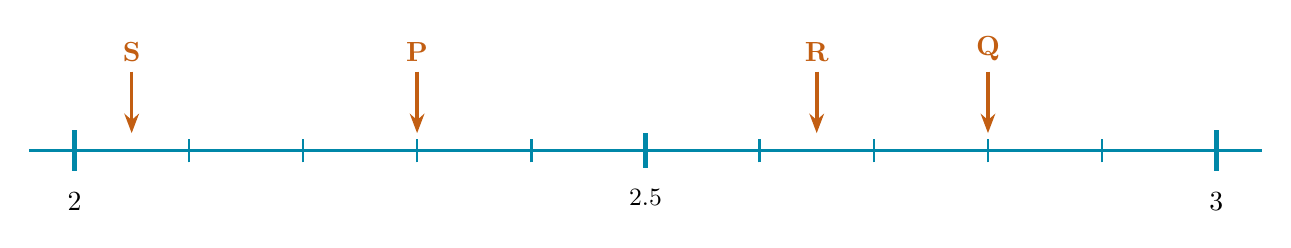
\begin{tikzpicture}[x=1.45cm, y=1cm, line width=0.9pt]
  \draw[cbteal] (-0.4,0) -- (10.4,0);
  \foreach \n in {0,...,10}{\draw[cbteal] (\n,-0.15) -- (\n,0.15);}
  \draw[cbteal, line width=1.6pt] (0,-0.26) -- (0,0.26);
  \draw[cbteal, line width=1.6pt] (5,-0.22) -- (5,0.22);
  \draw[cbteal, line width=1.6pt] (10,-0.26) -- (10,0.26);
  \node[below=4pt, font=\bfseries] at (0,-0.26) {$2$};
  \node[below=4pt, font=\small] at (5,-0.22) {$2.5$};
  \node[below=4pt, font=\bfseries] at (10,-0.26) {$3$};
  \foreach \x/\l in {3/P, 8/Q, 6.5/R, 0.5/S}{
    \draw[cborange, line width=1.3pt, -{Stealth[length=7pt]}] (\x,1.0) -- (\x,0.22);
    \node[above, font=\bfseries, text=cborange] at (\x,1.0) {\l};}
\end{tikzpicture}
\end{center}

\vspace{2pt}
\noindent
\begin{tabularx}{\textwidth}{|C{2.3cm}|C{2.3cm}|C{2.3cm}|C{2.3cm}|X}
  \cline{1-4}
  \textbf{P} \; \blank[1.3cm] \tall & \textbf{Q} \; \blank[1.3cm] &
  \textbf{R} \; \blank[1.3cm] & \textbf{S} \; \blank[1.3cm] & \\
  \cline{1-4}
\end{tabularx}

\vspace{6pt}
\noindent\begin{minipage}{\textwidth}
\textbf{(b)} Write the four numbers in order, \textbf{starting with the largest}
(the biggest).
\fr{(b) Range les quatre nombres dans l'ordre d\'ecroissant, du plus grand au plus
petit (\eng{starting with the largest}).}
\ansline[9.0cm]
\end{minipage}

% -- A2 ---------------------------------------------------------------------
\qhead{A2}{Which is bigger?\frin{Lequel est le plus grand~?}}

\noindent\begin{minipage}{\textwidth}
Write $<$, $>$ or $=$ in each box. Look at the whole-number parts first. Then
\key{fill with zeros}: \; $0.5 = 0.50$.
\fr{\'Ecris $<$, $>$ ou $=$ dans chaque case. Compare d'abord les parties enti\`eres,
puis ajoute des z\'eros (\eng{fill with zeros})~: $0.5 = 0.50$.}

\vspace{4pt}
\begin{multicols}{3}
\begin{enumerate}[label=(\alph*), itemsep=11pt]
  \item $0.5 \;\nbox\; 0.45$
  \item $2.1 \;\nbox\; 2.09$
  \item $8.08 \;\nbox\; 8.8$
  \item $6.4 \;\nbox\; 6.400$
  \item $15.6 \;\nbox\; 9.87$
  \item $1.25 \;\nbox\; 1.3$
\end{enumerate}
\end{multicols}
\end{minipage}

% -- A3 ---------------------------------------------------------------------
\qhead{A3}{Line up the points}

\begin{remember}[Written method]
  Write the numbers with the \key{points in a line}. Fill the gaps with
  \key{zeros}. The point in the answer goes \key{straight down}.
  \fr{Pose le calcul en colonnes, virgule sous virgule, et compl\`ete avec des
  z\'eros. Dans le r\'esultat, la virgule descend tout droit (\eng{straight
  down}).}
\end{remember}

\vspace{4pt}
\noindent
\wsq[\frl{2.4cm}{2.9cm}]{a}{7.8 + 4.56}\hfill\wsq[\frl{2.4cm}{2.9cm}]{b}{23.4 + 0.87 + 5}\hfill\wsq[\frl{2.4cm}{2.9cm}]{c}{16.25 + 3.9}

\vspace{4pt}
\noindent
\wsq[\frl{2.4cm}{2.9cm}]{d}{10 - 3.42}\hfill\wsq[\frl{2.4cm}{2.9cm}]{e}{6.3 - 2.75}\hfill\wsq[\frl{2.4cm}{2.9cm}]{f}{0.9 - 0.36}

% ===========================================================================
% SECTION B -- UNIT 4 REVIEW: 4.3, 4.4 AND THE 2-DIGIT REVIEW
% ===========================================================================
\hwsection{Section B \textperiodcentered\ Unit 4 Review --- Multiplying and Dividing}

\begin{remember}[Where the point goes]
  $\times$\,: take the point out and multiply, then \key{estimate} to put it back.
  \; $3.8 \times 12$: \; $38 \times 12 = 456$, and $4 \times 12 = 48$, so
  \key{45.6}. \\
  $\div$\,: short division. The point goes \key{straight up}. If a digit is too
  small to divide, write \key{0}. To divide by a 2-digit number, write its
  \key{times table} first.
  \fr{Multiplie sans la virgule, puis remets-la gr\^ace \`a l'estimation
  (\eng{estimate}). En division, la virgule monte tout droit (\eng{straight up})~;
  par un nombre \`a 2 chiffres, \'ecris d'abord sa table (\eng{times table}).}
\end{remember}

% -- B1 ---------------------------------------------------------------------
\qhead{B1}{Point out, point back}

\noindent\begin{minipage}{\textwidth}
Fill in the table. The first one is done for you.
\fr{Compl\`ete le tableau. La premi\`ere ligne est faite pour toi.}

\vspace{4pt}
\noindent
\begin{tabularx}{\textwidth}{|C{2.6cm}|L|C{3.5cm}|C{2.4cm}|}
  \hline
  \textbf{Calculation} & \textbf{Estimate} & \textbf{Without the point} &
  \textbf{Answer} \\
  \hline
  $2.4 \times 13$ \tall & $2 \times 13 = 26$ & $24 \times 13 = 312$ & $31.2$ \\ \hline
  $0.6 \times 9$ \tall & & & \\ \hline
  $3.45 \times 6$ \tall & & & \\ \hline
  $7.2 \times 15$ \tall & & & \\ \hline
  $2.8 \times 23$ \tall & & & \\ \hline
\end{tabularx}
\end{minipage}

% -- B2 ---------------------------------------------------------------------
% (b) and (c) need zeros in the answer; (d) runs out of digits; (e) and (f)
% are by a 2-digit number, with the table to write.
\qhead{B2}{The point goes straight up}

% The instruction is kept with the first row only, so the second row can go
% over a page break on its own.
\noindent\begin{minipage}{\textwidth}
Use short division. For \textbf{(e)} and \textbf{(f)}, write the times table first.
\fr{Pose les divisions. Pour (e) et (f), \'ecris d'abord la table de
multiplication.}

\vspace{4pt}
\noindent
\wsq[2.45cm]{a}{9.45 \div 5}\hfill\wsq[2.45cm]{b}{4.32 \div 4}\hfill\wsq[2.45cm]{c}{0.72 \div 9}
\end{minipage}

\vspace{4pt}
\noindent
\wsq[2.9cm]{d}{7.3 \div 2}\hfill\wsq[2.9cm]{e}{52.5 \div 15}\hfill\wsq[2.9cm]{f}{81.6 \div 24}

% ===========================================================================
% SECTION C -- UNIT 4 REVIEW: THE WORDS, 4.5 AND MONEY
% ===========================================================================
% Laid out by the page: C1 and its word help are one page, so no trap word is
% glossed on the other side of the sheet from its question; C2-C5 are the next.
% The French copy needs the whole of a page for C1, so it starts one.
\iffr\clearpage\fi
\hwsection{Section C \textperiodcentered\ Unit 4 Review --- Words, Quick Ways and Money}

% -- C1 ---------------------------------------------------------------------
% THE HEART OF THE MATHS. The numbers are easy on purpose; every item is
% decided by its English. (a) says "add" and is a subtraction. (d) puts the
% numbers in the opposite order to the sentence. (c) is two steps, and
% "altogether" is the second one. (b) is the review's 2-digit division.
\qhead{C1}{From English to a calculation}

\begin{wordhelp}[Word help --- the words that choose the operation]
  \begin{tabularx}{\linewidth}{@{}l@{\hspace{16pt}}X@{}}
    \eng{each} & for one of them. \emph{3 pens at 2 dollars each}: $3 \times 2$
      \frin{chacun} \\
    \eng{altogether} & all of it, the total \frin{en tout} \\
    \eng{twice as far} & 2 times as far \frin{deux fois plus loin} \\
    \eng{what must you add to 4 to make 7?} & $7 - 4$. It says \emph{add}, but
      you \textbf{subtract} \frin{que faut-il ajouter \`a 4 pour obtenir 7~?} \\
    \eng{3 less than 10} & $10 - 3$. The \textbf{second} number comes
      \textbf{first} \frin{3 de moins que 10} \\
  \end{tabularx}
\end{wordhelp}

\vspace{2pt}
\noindent Write the \textbf{calculation first}, then the answer. Give units.
\fr{\'Ecris d'abord le calcul (\eng{calculation}), puis le r\'esultat avec son
unit\'e.}

\begin{enumerate}[label=(\alph*), itemsep=6pt]
  \item What must you add to 4.65 to make 7?
        \fr{Que faut-il ajouter \`a 4.65 pour obtenir 7~?}
        \calcans
  \item A ribbon 2.4 m long is cut into 16 equal pieces. How long is each piece?
        \fr{On coupe un ruban de 2.4 m en 16 morceaux \'egaux. Quelle est la
        longueur de chaque morceau~?}
        \calcans
  \item Mr Bowen walks 2.5 km on Monday. On Tuesday he walks twice as far. How far
        does he walk altogether?
        \fr{Lundi, Mr Bowen marche 2.5 km. Mardi, il marche deux fois plus loin
        (\eng{twice as far}). Quelle distance parcourt-il en tout
        (\eng{altogether})~?}
        \calcans
  \item What is 3.5 less than 10?
        \fr{Combien font 3.5 de moins que 10 (\eng{3.5 less than 10})~?}
        \calcans
\end{enumerate}

% -- C2 ---------------------------------------------------------------------
\qhead{C2}{Use a quick way}

\begin{remember}[Quick ways]
  $\times\, 0.5$ = \key{half of} \quad $\times\, 0.25$ = \key{a quarter of} \quad
  $\times\, 0.07$ = $\div\, 100$, then $\times\, 7$ \\
  $\times\, 9$: $\times\, 10$, then \key{take away} one lot. \quad
  $\times\, 11$: $\times\, 10$, then \key{add} one lot. \\
  \key{Partitioning}: split the number. \; $4.3 \times 6 = 24 + 1.8$
  \fr{\eng{half of} = la moiti\'e de~; \eng{a quarter of} = le quart de. $\times 9$~:
  multiplie par 10, puis retire le nombre une fois~; $\times 11$~: multiplie par
  10, puis ajoute-le une fois. \eng{Partitioning}~: d\'ecomposer le nombre.}
\end{remember}

\vspace{2pt}
\noindent Write the quick way, then the answer.
\fr{\'Ecris le calcul rapide, puis le r\'esultat.}

\vspace{4pt}
\begin{multicols}{2}
\begin{enumerate}[label=(\alph*), itemsep=12pt]
  \item $4.7 \times 9 = \blank[2.6cm] = \blank[1.4cm]$
  \item $6.2 \times 11 = \blank[2.6cm] = \blank[1.4cm]$
  \item $5.3 \times 4 = \blank[2.6cm] = \blank[1.4cm]$
  \item $64 \times 0.25 = \blank[2.4cm] = \blank[1.4cm]$
  \item $300 \times 0.07 = \blank[2.2cm] = \blank[1.4cm]$
  \item $9.6 \times 0.5 = \blank[2.6cm] = \blank[1.4cm]$
\end{enumerate}
\end{multicols}

% -- C3 ---------------------------------------------------------------------
% Four steps, and money to 2 d.p. A minipage, so the question cannot be left on
% one page with its box on the next.
\qhead{C3}{Change from 10 dollars}

\noindent\begin{minipage}{\textwidth}
Money has \key{2 decimal places}: 7.8 dollars is written 7.80 dollars.
\fr{Une somme d'argent s'\'ecrit avec 2 chiffres apr\`es la virgule (\eng{2 decimal
places})~: 7.8 dollars s'\'ecrit 7.80 dollars.}

\vspace{4pt}
\noindent Mr Bowen buys 3 b\'anh m\`{\i} at 1.35 dollars each and 2 iced coffees at
1.90 dollars each. He pays with a 10-dollar note. How much change does he get?
\fr{Mr Bowen ach\`ete 3 b\'anh m\`{\i} \`a 1.35 dollar chacun et 2 caf\'es glac\'es
\`a 1.90 dollar chacun. Il paie avec un billet de 10 dollars. Combien de monnaie
(\eng{change}) lui rend-on~?}
\begin{workspace}[\frl{2.7cm}{3.2cm}]\end{workspace}
\end{minipage}

% -- C4 ---------------------------------------------------------------------
% One trap each from 4.2, 4.4, 4.1 and 4.5. See the key.
\qhead{C4}{Mr Bowen's homework}

\noindent\begin{minipage}{\textwidth}
Only \textbf{one} of these is right. Find it, and correct the other three.
\fr{Une seule r\'eponse est juste~: trouve-la, puis corrige les trois autres.}

\vspace{4pt}
\begin{multicols}{2}
\begin{enumerate}[label=(\alph*), itemsep=12pt]
  \item $4.5 + 2.7 = 6.12$ \; \blank[2.2cm]
  \item $9.6 \div 3 = 3.2$ \; \blank[2.2cm]
  \item $3.40 > 3.4$ \; \blank[2.2cm]
  \item $60 \times 0.4 = 2.4$ \; \blank[2.2cm]
\end{enumerate}
\end{multicols}
\end{minipage}

% -- C5 ---------------------------------------------------------------------
% Calculation -> English. A minipage: the rules and the expression were split
% across a page on one build.
\qhead{C5}{Now you write the question}

\noindent\begin{minipage}{\textwidth}
\begin{yourturn}[The rules]
  A \textbf{real} situation, in full sentences, ending in a \textbf{question}. Use
  a \eng{word} from C1, give \textbf{units}, and come out at the answer given.
  \fr{Une situation de la vie r\'eelle, des phrases compl\`etes, une question \`a la
  fin, un mot de C1 et des unit\'es. \textbf{\'Ecris ton probl\`eme en anglais.}}
\end{yourturn}

\vspace{4pt}
\noindent Write a word problem for \quad \expr{12 \times 2.40 = 28.80}
\fr{Invente, en anglais, un probl\`eme (\eng{word problem}) qui correspond \`a ce
calcul.}
\wlines{\frl{3}{4}}
\end{minipage}

% ===========================================================================
% SECTION D -- SCIENCE 3.2 AND MODELS PART 1: HOW THE SOLAR SYSTEM FORMED
% ===========================================================================
\hwsection[cbgreen]{Section D \textperiodcentered\ Science 3.2 --- How the Solar System Formed}

% -- D1 ---------------------------------------------------------------------
\qhead[cbgreen]{D1}{Key words}

\noindent\begin{minipage}{\textwidth}
Write the letter of the right meaning next to each word.
\fr{\'Ecris \`a c\^ot\'e de chaque mot la lettre de sa d\'efinition.}

\vspace{6pt}
\noindent
\begin{tabularx}{\textwidth}{|>{\bfseries\color{cbblue}}l|C{1.3cm}|C{0.7cm}|L|}
  \hline
  nebula \tall & & \textbf{A} & an idea that can be tested
    \frin{une id\'ee qu'on peut tester} \\ \hline
  hypothesis \tall & & \textbf{B} & one flat surface \frin{une seule surface
    plate} \\ \hline
  evidence \tall & & \textbf{C} & a cloud of dust and gas in space \frin{un nuage
    de poussi\`ere et de gaz} \\ \hline
  model \tall & & \textbf{D} & facts from observations or experiments \frin{des
    faits tir\'es d'observations ou d'exp\'eriences} \\ \hline
  limitation \tall & & \textbf{E} & something a model cannot do, gets wrong or
    leaves out \frin{ce qu'un mod\`ele ne peut pas faire, montre mal ou oublie} \\
    \hline
  plane \tall & & \textbf{F} & a way of showing something that is hard to observe
    directly \frin{une fa\c{c}on de montrer ce qu'on ne peut pas bien observer} \\
    \hline
\end{tabularx}
\end{minipage}

% -- D2 ---------------------------------------------------------------------
% Four facts support, two contradict. (b) is the deck's Question 4: most, but
% not all, of the evidence supports it, so it is not thrown out.
\qhead[cbgreen]{D2}{Support or contradict?}

\noindent\begin{minipage}{\textwidth}
\noindent The \textbf{hypothesis}: \; \key{The Sun and the planets formed from one
spinning cloud of dust and gas.}
\fr{L'hypoth\`ese~: le Soleil et les plan\`etes viennent d'un seul nuage de
poussi\`ere et de gaz qui tournait.}

\vspace{6pt}
\noindent
\begin{tabularx}{\textwidth}{|L|C{2.5cm}|C{2.5cm}|}
  \hline
  Does each fact \textbf{support} the hypothesis, or \textbf{contradict} it? Tick
    one box.
    \fr{Chaque fait confirme-t-il (\eng{supports}) l'hypoth\`ese, ou la
    contredit-il (\eng{contradicts})~? Coche une case.}
    & \textbf{supports} & \textbf{contradicts} \\ \hline
  All the planets orbit the Sun in the same direction. \frin{m\^eme sens} & & \\
    \hline
  All the orbits are in the same plane. \frin{m\^eme plan} & & \\ \hline
  Venus spins the opposite way to most planets. \frin{sens oppos\'e} & & \\ \hline
  HL Tauri is a young star with a flat disc of dust round it. \frin{un disque
    plat} & & \\ \hline
  Uranus spins on its side. \frin{sur le c\^ot\'e} & & \\ \hline
  Most moons orbit their planet in the same direction. \frin{la plupart des
    lunes} & & \\ \hline
\end{tabularx}
\end{minipage}

\vspace{8pt}
\noindent\begin{minipage}{\textwidth}
\textbf{(b)} Two facts contradict the hypothesis. So is it wrong? Answer in a full
sentence. Use the words \eng{most of the evidence}.
\fr{(b) Deux faits contredisent l'hypoth\`ese. Est-elle donc fausse~? R\'eponds par
une phrase compl\`ete, en anglais, avec les mots \eng{most of the evidence}.}
\wlines{\frl{2}{4}}
\end{minipage}

% -- D3 ---------------------------------------------------------------------
% (a) is the Models deck's four-step write note, shuffled. (c) is its "Rocky or
% giant?" slide. (d) is 3.2's 99.8%, as a decimal subtraction.
\iffr\clearpage\fi
\qhead[cbgreen]{D3}{From a cloud to the Sun and planets}

\noindent\begin{minipage}{\textwidth}
\textbf{(a)} Put the four steps in order. Write \textbf{1}, \textbf{2}, \textbf{3}
and \textbf{4} in the boxes.
\fr{(a) Remets les quatre \'etapes dans l'ordre~: \'ecris 1, 2, 3 et 4 dans les
cases.}

\vspace{4pt}
\renewcommand{\arraystretch}{1.6}%
\noindent
\begin{tabular}{@{}c@{\hspace{10pt}}l@{}}
  \nbox & The hot middle becomes the Sun. \frin{le centre chaud devient le Soleil} \\
  \nbox & Gravity pulls the nebula together. It spins faster. \frin{la gravit\'e
    rassemble la n\'ebuleuse} \\
  \nbox & Dust sticks together and grows into planets. \frin{la poussi\`ere forme des
    plan\`etes} \\
  \nbox & The nebula flattens into a spinning disc. \frin{la n\'ebuleuse s'aplatit en disque} \\
\end{tabular}
\renewcommand{\arraystretch}{1.45}%
\end{minipage}

\vspace{8pt}
\noindent\begin{minipage}{\textwidth}
\textbf{(b)} Why do all the planets orbit the Sun in the same direction? Answer in a
full sentence. \; Start: \eng{``They all formed from \ldots''}
\fr{(b) Pourquoi toutes les plan\`etes tournent-elles autour du Soleil dans le m\^eme
sens~? R\'eponds par une phrase compl\`ete, en anglais.}
\wlines{\frl{2}{4}}
\end{minipage}

\vspace{6pt}
\noindent\begin{minipage}{\textwidth}
\textbf{(c)} Mercury, Venus, the Earth and Mars are small and rocky. Why? \;
Start: \eng{``Near the Sun, it was too hot for \ldots''}
\fr{(c) Mercure, V\'enus, la Terre et Mars sont petites et rocheuses. Pourquoi~?
R\'eponds en anglais.}
\wlines{\frl{2}{4}}
\end{minipage}

\vspace{6pt}
\noindent\textbf{(d)} The Sun has \textbf{99.8\%} of all the mass in the Solar
System. \% means \emph{out of 100}. How many \% are left for everything else?
\hfill \blank[2.4cm]
\fr{(d) Le Soleil a 99.8\,\% de toute la masse du syst\`eme solaire (\% = sur 100).
Quel pourcentage reste-t-il pour tout le reste~?}

% ===========================================================================
% SECTION E -- SCIENCE 3.3: MOVEMENT IN SPACE
% ===========================================================================
\iffr\clearpage\fi
\hwsection[cbgreen]{Section E \textperiodcentered\ Science 3.3 --- Movement in Space}

% -- E1 ---------------------------------------------------------------------
% The deck's vote and its Draw This, on paper. (c) is the vote: the planet goes
% STRAIGHT ON (along the tangent, up the page), not outwards (to the right).
% The arrows on the orbit say which way it moves, so (c) has one answer.
% One minipage from the drawing to (c): (b) and (c) are drawn on it, and the
% French copy put (c) on the next page.
\qhead[cbgreen]{E1}{What keeps a planet in orbit?}

\noindent\begin{minipage}{\textwidth}
\textbf{(a)} Label the drawing. Use these words: \; \eng{Sun} \sep \eng{orbit}
\sep \eng{planet}
\fr{(a) Compl\`ete les \'etiquettes avec ces mots~: \eng{Sun} (le Soleil), \eng{orbit}
(l'orbite), \eng{planet} (la plan\`ete).}

\vspace{2pt}
\begin{center}
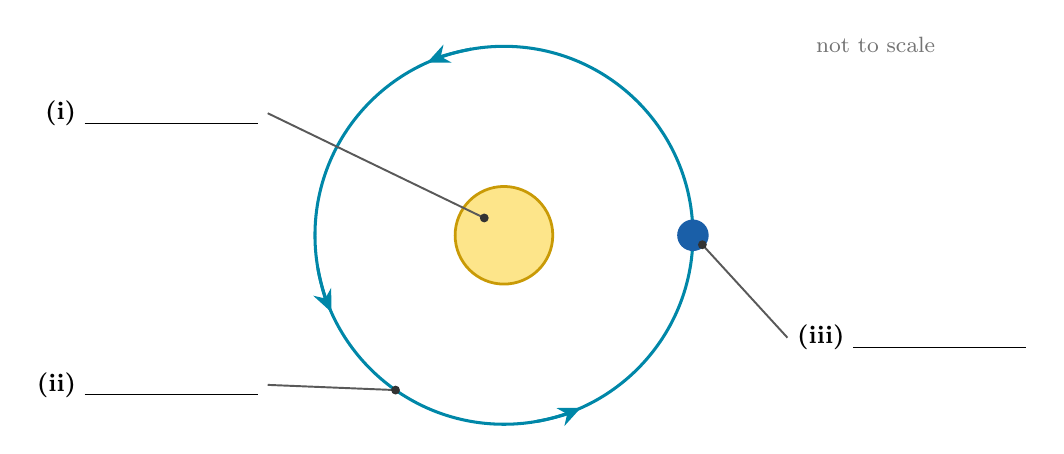
\begin{tikzpicture}[x=1cm, y=1cm]
  % orbit, with three arrowheads: the planet goes anticlockwise
  \draw[cbteal, line width=1.1pt] (0,0) circle (2.4);
  \foreach \a in {100, 190, 280}
    \draw[cbteal, line width=1.1pt, -{Stealth[length=8pt, width=7pt]}]
      (\a:2.4) arc (\a:\a+14:2.4);
  % Sun
  \fill[sunfill] (0,0) circle (0.62);
  \draw[sunrim, line width=1pt] (0,0) circle (0.62);
  % planet, at 3 o'clock
  \fill[cbblue] (2.4,0) circle (0.2);
  % leader lines, each ending on a dot on its target
  \draw[black!65, line width=0.7pt] (-0.25,0.22) -- (-3.0,1.55);
  \fill[black!80] (-0.25,0.22) circle (1.6pt);
  \node[left, font=\small] at (-3.0,1.55) {\textbf{(i)} \blank[2.2cm]};
  \draw[black!65, line width=0.7pt] (235:2.4) -- (-3.0,-1.9);
  \fill[black!80] (235:2.4) circle (1.6pt);
  \node[left, font=\small] at (-3.0,-1.9) {\textbf{(ii)} \blank[2.2cm]};
  \draw[black!65, line width=0.7pt] (2.52,-0.12) -- (3.6,-1.3);
  \fill[black!80] (2.52,-0.12) circle (1.6pt);
  \node[right, font=\small] at (3.6,-1.3) {\textbf{(iii)} \blank[2.2cm]};
  \node[font=\footnotesize, text=black!55, anchor=south east] at (5.6,2.2)
    {not to scale};
\end{tikzpicture}
\end{center}

\vspace{4pt}
\begin{enumerate}[label=(\alph*), start=2, itemsep=6pt]
  \item Draw an \textbf{arrow} on the planet to show the pull of the Sun's
        \textbf{gravity}.
        \fr{Dessine sur la plan\`ete une fl\`eche qui montre l'attraction de la
        gravit\'e du Soleil.}
  \item The arrows show which way the planet moves. Now the Sun's gravity
        \textbf{switches off}. Draw a \textbf{dashed line} to show where the planet
        goes.
        \fr{Les fl\`eches sur l'orbite montrent le sens du mouvement. La gravit\'e du
        Soleil s'arr\^ete (\eng{switches off})~: trace en pointill\'es
        (\eng{dashed line}) le chemin de la plan\`ete.}
\end{enumerate}
\end{minipage}

% -- E2 ---------------------------------------------------------------------
% Rows 1-2 are the deck's Question 6 (gravity only: space is a vacuum). Rows 3
% and 4 are on Earth, where there is air: the 3.1 lab's balcony drop and the
% landing plane from the air resistance slide.
% No word-help box: "vacuum" is what (b) asks for, and both words are the
% lesson's own write notes.
\qhead[cbgreen]{E2}{Which forces?\frin{Quelles forces~?}}

\noindent\begin{minipage}{\textwidth}
\noindent
\begin{tabularx}{\textwidth}{|L|C{2.6cm}|C{2.6cm}|}
  \hline
  Which forces act on each one? Tick \textbf{every} box that is true.
    \fr{Quelles forces agissent sur chacun~? Coche toutes les cases justes.}
    & \textbf{gravity} & \textbf{air resistance} \\ \hline
  The Earth, orbiting the Sun \frin{la Terre} \tall & & \\ \hline
  The Moon, orbiting the Earth \frin{la Lune} \tall & & \\ \hline
  A ball falling from the balcony \frin{une balle qui tombe} \tall & & \\ \hline
  A plane landing on a runway \frin{un avion qui atterrit} \tall & & \\ \hline
\end{tabularx}
\end{minipage}

\vspace{8pt}
\noindent\begin{minipage}{\textwidth}
\textbf{(b)} Why do the planets never slow down? \; Start: \eng{``Space is a
\ldots, so \ldots''}
\fr{(b) Pourquoi les plan\`etes ne ralentissent-elles jamais~? R\'eponds par une
phrase compl\`ete, en anglais.}
\wlines{2}
\end{minipage}

% ===========================================================================
% SECTION F -- WHERE THEY MEET: FASTER NEAR THE SUN
% ===========================================================================
\hwsection[cbgreen]{Section F \textperiodcentered\ Science in Decimals --- Faster Near the Sun}

\begin{remember}[Speed, from Science 3.3]
  \key{Speed}: how fast something moves. \; \key{km/s} = kilometres \key{per}
  second. \\
  As the distance from the Sun \key{increases}, the speed of the planets
  \key{decreases}. The Sun's pull is \key{weaker} far away.
  \fr{Vitesse (\eng{speed})~: la rapidit\'e d'un mouvement. km/s = kilom\`etres par
  seconde. Plus une plan\`ete est loin du Soleil, plus elle est lente~:
  l'attraction du Soleil est plus faible (\eng{weaker}) au loin.}
\end{remember}

% -- F1 ---------------------------------------------------------------------
% The pair that looks identical and is not: how much faster (subtract) and how
% many times as fast (divide), on the same two planets, in the same row.
\qhead[cbgreen]{F1}{How much faster? How many times as fast?}

% The speeds from the lesson (the book's Activity table). One minipage down to
% the end of the table to fill in: the speeds, the word help and the questions
% must be on one page (the French copy split them).
\noindent\begin{minipage}{\textwidth}
\begin{center}
\setlength{\tabcolsep}{3pt}%
\begin{tabular}{|l|*{8}{C{1.50cm}|}}
  \hline
  & \small Mercury & \small Venus & \small Earth & \small Mars & \small Jupiter &
  \small Saturn & \small Uranus & \small Neptune \\
  \hline
  \textbf{speed} (km/s) & \textbf{48} & \textbf{35} & \textbf{30} & \textbf{24} &
  \textbf{13} & \textbf{10} & \textbf{7} & \textbf{5} \\
  \hline
\end{tabular}
\end{center}

\vspace{4pt}
\begin{wordhelp}[Word help --- two questions that look the same]
  \begin{tabularx}{\linewidth}{@{}l@{\hspace{16pt}}X@{}}
    \eng{how much faster?} & the difference. \textbf{Subtract} \frin{de combien
      plus rapide~? = la diff\'erence} \\
    \eng{how many times as fast?} & \textbf{divide} the bigger speed by the smaller
      one \frin{combien de fois plus rapide~? = une division} \\
  \end{tabularx}
\end{wordhelp}

\vspace{2pt}
\noindent
\begin{tabularx}{\textwidth}{|L|C{4.5cm}|C{4.5cm}|}
  \hline
  Fill in the table. The first row is done for you.
    \fr{Compl\`ete le tableau. La premi\`ere ligne est faite pour toi.}
    & \textbf{How much faster?} & \textbf{How many times as fast?} \\
  \hline
  Mercury and Neptune \tall & $48 - 5 = 43$ km/s & $48 \div 5 = 9.6$ \\ \hline
  Mercury and the Earth \tall & & \\ \hline
  Mars and Saturn \tall & & \\ \hline
  The Earth and Mars \tall & & \\ \hline
\end{tabularx}
\end{minipage}

% -- F2 ---------------------------------------------------------------------
% The football model from Models Part 1. (a) is a units trap: 2.3 cm is bigger
% than 7.8 mm. (b) is the deadpan one, and needs only the deck's 24 m.
% The table and (a) are one minipage: (a) cannot be done without the table.
\iffr\clearpage\fi
\qhead[cbgreen]{F2}{The Sun is a football}

\noindent\begin{minipage}{\textwidth}
In the lesson the Sun became a football, and everything else shrank by the same
amount.
\fr{En classe, le Soleil est devenu un ballon de foot, et tout le reste a \'et\'e
r\'eduit de la m\^eme fa\c{c}on.}

\vspace{6pt}
{\centering
\setlength{\tabcolsep}{5pt}%
\begin{tabular}{|l|*{5}{C{1.95cm}|}}
  \hline
  & \textbf{the Moon} & \textbf{the Earth} & \textbf{Neptune} & \textbf{Jupiter} &
  \textbf{the Sun} \\ \hline
  \textbf{Model width} & 0.5 mm & 2 mm & 7.8 mm & 2.3 cm & 22 cm \\ \hline
  \textbf{Like} & \small a grain of sand & \small a pinhead & \small a pea &
  \small a grape & \small a football \\ \hline
\end{tabular}\par}

\vspace{6pt}
\noindent\textbf{(a)} Write the five model widths in order of size, starting with
the \textbf{smallest}. Remember: \mbox{\key{1 cm = 10 mm}}.
\fr{(a) Range les cinq largeurs dans l'ordre croissant, de la plus petite \`a la
plus grande (1 cm = 10 mm).}
\ansline[11.0cm]
\end{minipage}

\begin{enumerate}[label=(\alph*), start=2, itemsep=6pt]
  \item In the model, the Earth is \textbf{24 m} from the football. Mr Bowen builds
        the model in his classroom, which is \textbf{8.5 m} long. He puts the
        football against one wall. How far past the other wall must the Earth go?
        \fr{Dans le mod\`ele, la Terre est \`a 24 m du ballon. Mr Bowen construit le
        mod\`ele dans sa classe, qui mesure 8.5 m de long. Il pose le ballon contre
        un mur. \`A quelle distance derri\`ere l'autre mur doit-il mettre la Terre~?}
        \iffr\par\nobreak\begin{workspace}[2.2cm]\end{workspace}\fi
        \calcans
  \item Give \textbf{one limitation} of the football model. \; Start:
        \eng{``One limitation of the football model is \ldots''}
        \fr{Donne une limite (\eng{limitation}) du mod\`ele du ballon de foot, en
        anglais.}
        \qlines{\frl{2}{4}}
\end{enumerate}

% -- F3 ---------------------------------------------------------------------
% THE KEYSTONE, and last. 3.3's exit question with NASA's numbers. (b) is
% 3.3's reason, in a sentence: closer, so a stronger pull. (d)-(e): the mean is
% 29.8, which rounds to the book's 30. (e) quotes the 30 so it does not send
% the student back a page to F1. The whole question is one block: every part
% reads the table.
\qhead[cbgreen]{F3}{Faster in January}

\noindent\begin{minipage}{\textwidth}
The Earth's orbit is \emph{almost} circular. In January the Earth is a little
\textbf{closer} to the Sun than in July.
\fr{L'orbite de la Terre est \emph{presque} circulaire. En janvier, la Terre est un
peu plus proche (\eng{closer}) du Soleil qu'en juillet.}

\vspace{6pt}
{\centering
\begin{tabular}{|l|C{4.4cm}|C{3.2cm}|}
  \hline
  & \textbf{Distance from the Sun} & \textbf{Speed} \\ \hline
  \textbf{January} & 147.1 million km & 30.3 km/s \\ \hline
  \textbf{July}    & 152.1 million km & 29.3 km/s \\ \hline
\end{tabular}\par}

\vspace{4pt}
\begin{enumerate}[label=(\alph*), itemsep=6pt]
  \item How much closer to the Sun is the Earth in January?
        \fr{De combien la Terre est-elle plus proche du Soleil en janvier~?}
        \calcans
  \item In which month is the Earth faster? Why? Use the words \eng{closer} and
        \eng{pull}. \; Start: \eng{``The Earth is faster in \ldots, because
        \ldots''}
        \fr{En quel mois la Terre va-t-elle le plus vite~? Pourquoi~? R\'eponds par
        une phrase compl\`ete, en anglais, avec les mots \eng{closer} et
        \eng{pull}.}
        \qlines{3}
  \item How much faster is the Earth in January than in July?
        \fr{De combien la Terre va-t-elle plus vite en janvier qu'en juillet~?}
        \calcans
  \item Find the \textbf{mean} of the two speeds. \frin{la moyenne}
        \calcans
  \item Round your mean to the nearest whole number. \hfill \blank[2.6cm]
        \fr{Arrondis ta moyenne \`a l'unit\'e.}
        \par\vspace{6pt}
        In the lesson, the Earth's speed was \textbf{30 km/s}. What do you notice?
        \fr{En classe, la vitesse de la Terre \'etait de 30 km/s. Que remarques-tu~?
        R\'eponds en anglais.}
        \qlines{2}
\end{enumerate}
\end{minipage}

% ===========================================================================
% ANSWER KEY -- TEACHER COPY ONLY
% ===========================================================================
\ifkey
\clearpage

\hwsection[cbred]{Answer Key --- Teacher Copy}

\linespread{1.0}\selectfont
\setlist[enumerate]{itemsep=2pt, topsep=3pt, leftmargin=*}
\setlist[itemize]{itemsep=2pt, topsep=3pt, leftmargin=*}

\qhead[cbred]{A1}{Read the line}
\noindent (a) P $2.3$ \sep Q $2.8$ \sep R $2.65$ \sep S $2.05$ \\
(b) $2.8, \; 2.65, \; 2.3, \; 2.05$

\smallskip
\noindent{\small R and S sit halfway between two lines; HW 9's A1 asked the class to
\emph{place} 5.45 and 5.05, and this asks them to \emph{read} them. Expect $2.5$ for
S from a student who sees ``halfway'' and writes a 5 in the tenths, and $2.6$ or
$2.7$ for R.
(b) runs from the \emph{largest} on purpose --- HW 9 always ran from the smallest.
A list that starts with $2.05$ is right in the wrong direction: ask what
\emph{largest} means.}

\qhead[cbred]{A2}{Which is bigger?}
\noindent (a) $>$ \quad (b) $>$ \quad (c) $<$ \quad (d) $=$ \quad (e) $>$ \quad
(f) $<$

\smallskip
\noindent{\small (a) and (f) are the same trap from two sides: the number with more
digits is the smaller one ($0.50 > 0.45$, $1.25 < 1.30$). (c) is ``eight point zero
eight'' against ``eight point eight''; anyone who reads both as ``eight point eight''
has dropped the zero. (e) is the whole-number part first: $15 > 9$, and the
digits after the point do not matter.}

\qhead[cbred]{A3}{Line up the points}
\noindent (a) $12.36$ \quad (b) $29.27$ \quad (c) $20.15$ \quad (d) $6.58$ \quad
(e) $3.55$ \quad (f) $0.54$

\smallskip
\noindent{\small (a) and (c) are the alignment check: lining up the right-hand digits
gives $7.8 + 4.56 = 5.34$ and $16.25 + 3.9 = 16.64$. (b) has a whole number with no
point: $5 = 5.00$. (d), (e) and (f) need the zeros \emph{written} first: $10.00$,
$6.30$, $0.90$. Expect $7.42$ for (d) from a student who took $10 - 3$ and copied the
$.42$.}

\qhead[cbred]{B1}{Point out, point back}
\noindent
\begin{tabular}{@{}llll@{}}
  $0.6 \times 9$ & $1 \times 9 = 9$ & $6 \times 9 = 54$ & $\mathbf{5.4}$ \\
  $3.45 \times 6$ & $3 \times 6 = 18$ & $345 \times 6 = 2070$ & $\mathbf{20.7}$ \\
  $7.2 \times 15$ & $7 \times 15 = 105$ & $72 \times 15 = 1080$ & $\mathbf{108}$ \\
  $2.8 \times 23$ & $3 \times 20 = 60$ & $28 \times 23 = 644$ & $\mathbf{64.4}$ \\
\end{tabular}

\smallskip
\noindent{\small Rows 2 and 3 end in a zero once the point is back ($20.70$,
$108.0$); accept them with or without it. Row 3 is the one to watch: $72 \times 15 =
1080$, and a student who puts back a place for \emph{each} number writes $10.80$.
Only $7.2$ has a decimal place. The estimate, 105, settles it. \\
Row 1 is $0.6 \times 9$, not $6 \times 9$: expect $0.54$ from anyone counting all
the digits instead of the decimal places. \\
Any sensible estimate is right ($2.8 \times 23 \approx 3 \times 23 = 69$ is fine).}

\qhead[cbred]{B2}{The point goes straight up}
\noindent (a) $1.89$ \quad (b) $\mathbf{1.08}$ \quad (c) $\mathbf{0.08}$ \quad
(d) $\mathbf{3.65}$ \quad (e) $3.5$ \quad (f) $3.4$

\smallskip
\noindent{\small (b) needs one 0 (4 into 3 will not go); expect $1.8$. (c) needs
two: 9 into 0, then 9 into 7, will not go. Expect $0.8$, which is $0.72 \div 0.9$. \\
(d) runs out of digits: write $7.30$ and keep going. ``$3.6$ remainder 1'' is the
usual stop. \\
(e) and (f): the table is the method. $15 \times 3 = 45$, $7.5$ left $= 15 \times
0.5$. \; $24 \times 3 = 72$, $9.6$ left $= 24 \times 0.4$. A student with the right
answer and no table probably knew it; one with a wrong answer and no table needs
telling to write the table.}

\qhead[cbred]{C1}{From English to a calculation}
\noindent (a) $7 - 4.65 = 2.35$ \quad (b) $2.4 \div 16 = 0.15$ m \\
(c) $2.5 \times 2 = 5$, \; $2.5 + 5 = \mathbf{7.5}$ km \quad (d) $10 - 3.5 = 6.5$

\smallskip
\noindent{\small \textbf{Mark the calculation, not the answer.} This is the English
question. \\
(a) says \emph{add} and is a subtraction. $4.65 + 7 = 11.65$ is the English error,
not an arithmetic one: have the student read the word-help line aloud. \\
(d) is ``3.5 less than 10'': $3.5 - 10$ is reading left to right. \\
(c) is two steps and \emph{altogether} is the second. Expect $5$ km, which is
Tuesday alone. \\
(b) is the 16 table: $16 \times 0.1 = 1.6$, $0.8$ left $= 16 \times 0.05$. Expect
$1.5$ from a student who did $24 \div 16$ and put the point back in the wrong place;
the estimate (2.4 m in 16 pieces is much less than 1 m each) catches it.}

\qhead[cbred]{C2}{Use a quick way}
\noindent (a) $47 - 4.7 = 42.3$ \quad (b) $62 + 6.2 = 68.2$ \quad
(c) $20 + 1.2 = 21.2$ \\
(d) a quarter of $64 = 16$ \quad (e) $3 \times 7 = 21$ \quad
(f) half of $9.6 = 4.8$

\smallskip
\noindent{\small (a) needs $47.0 - 4.7$. Expect $43.7$ from a student who took
$47 - 4$ and copied the $.7$ across --- the A3(d) error again. \\
(e) divides by \textbf{100}, not 10. Expect $210$ ($30 \times 7$). \\
Accept a correct written method for any of them, but the column is ``the quick way'':
ask for the quick way.}

\qhead[cbred]{C3}{Change from 10 dollars}
\noindent $3 \times 1.35 = 4.05$, \; $2 \times 1.90 = 3.80$, \; $4.05 + 3.80 =
7.85$, \; $10.00 - 7.85 = \mathbf{2.15}$ dollars

\smallskip
\noindent{\small Four steps. The usual slip is to stop at $7.85$ and call it the
change; ask what the question asked for. $3.8$ for the coffees is right but is money,
so $3.80$. \\
$10.00 - 7.85$ needs the zeros written. Expect $3.85$ from a student who took $10 -
7 = 3$ and copied the $.85$ --- A3(d) and C2(a) again.}

\qhead[cbred]{C4}{Mr Bowen's homework}
\noindent (a) \textbf{wrong} --- $7.2$. He added $4 + 2$ and $5 + 7$ separately; the
12 tenths carry. \\
(b) \textbf{right.} \\
(c) \textbf{wrong} --- $3.40 = 3.4$. The zero at the end does not change anything. \\
(d) \textbf{wrong} --- $24$. $\times\, 0.4$ is $\div\, 10$, then $\times\, 4$: $6
\times 4$.

\smallskip
\noindent{\small One trap each from 4.2, 4.4, 4.1 and 4.5. Whichever one a student
gets wrong, send them back to A3, B2, A2 or C2 rather than explaining again. \\
(b) is right on purpose and is the one with most room for doubt: a student who
expects every division to need a 0 will ``correct'' it to $3.02$.}

\qhead[cbred]{C5}{Now you write the question}
\noindent Check, in order: a real situation; full sentences; ends in a question
mark; uses a word from C1; gives units; and it really comes out at $28.80$.

\smallskip
\noindent{\small A good answer: ``Mr Bowen buys 12 notebooks at 2.40 dollars each.
How much does he pay altogether?'' \\
The common failure is a question whose answer is $0.20$: ``12 friends share 2.40
dollars''. Read it back to them and ask what the calculation in the box does. \\
Units need not be dollars --- ``12 bags of rice, 2.40 kg each'' is just as good ---
but $28.80$ with two decimal places is a strong hint.}

\qhead[cbred]{D1}{Key words}
\noindent nebula \textbf{C} \sep hypothesis \textbf{A} \sep evidence \textbf{D}
\sep model \textbf{F} \sep limitation \textbf{E} \sep plane \textbf{B}

\smallskip
\noindent{\small These are the 3.2 and Models write notes, word for word. Hypothesis
and evidence (A and D) are the pair most often swapped; \emph{plane} is the one most
often left blank (``not an aeroplane'').}

\qhead[cbred]{D2}{Support or contradict?}
\noindent Supports: rows 1, 2, 4, 6. \quad Contradicts: rows 3 (Venus), 5
(Uranus). \\
(b) ``No. Most of the evidence supports the hypothesis, so it is not wrong. It is
just not proven.''

\smallskip
\noindent{\small (b) is the deck's Question 4 (``most, but not all, of the evidence
supports it''). Accept any sentence that says the hypothesis is kept because most
evidence supports it. A student who says ``yes, it is wrong'' has heard
\emph{contradict} as \emph{prove wrong}; the cake on deck slide 6 is the
reminder --- two clues still supported the cat. \\
Row 4 (HL Tauri) is the one students hesitate over. It supports: a young star with a
flat disc is the hypothesis happening today.}

\qhead[cbred]{D3}{From a cloud to the Sun and planets}
\noindent (a) In the order printed: \textbf{3, 1, 4, 2}. \\
(b) ``They all formed from one spinning cloud, so they all still go round the same
way.'' \\
(c) ``Near the Sun, it was too hot for ice, so only rock and metal were left to make
planets.'' \\
(d) $100 - 99.8 = \mathbf{0.2}\%$

\smallskip
\noindent{\small (a) The printed order is shuffled; read it as ``the hot middle is
3''. The usual error is putting the Sun first, which is the order of importance, not
of time. \\
(c) is the Models deck's ``Rocky or giant?'' slide; ``too hot for ice'' is the
point. Accept ``too hot for gas'' only if they also say the planets are made of rock
and metal. \\
(d) needs $100.0 - 99.8$. Expect $1.8$ ($100 - 99$, then the $.8$ copied) or $1.2$
from anyone who did not write the zero. Every planet, moon, asteroid and comet together is two tenths of one percent:
that is worth saying aloud.}

\qhead[cbred]{E1}{What keeps a planet in orbit?}
\noindent (a) (i) Sun \sep (ii) orbit \sep (iii) planet \\
(b) An arrow from the planet pointing \textbf{to the left}, at the Sun. \\
(c) A straight dashed line going \textbf{straight up the page} from the planet ---
along the direction it was moving, touching the orbit, not crossing it.

\smallskip
\noindent{\small (c) is the class vote from the lesson (left hand ``away from the
centre'', right hand ``straight on''), and the wrong answer is the same here: a line
straight out to the right, away from the Sun. It means the student thinks something
was pushing the planet outwards. Nothing was --- gravity was pulling it in, and when
gravity stops the planet simply keeps going the way it was going. \\
A curved dashed line that keeps going round is the other error: without gravity
nothing turns it.}

\qhead[cbred]{E2}{Which forces?}
\noindent Earth: gravity \sep Moon: gravity \sep falling ball: gravity
\emph{and} air resistance \sep plane: gravity \emph{and} air resistance \\
(b) ``Space is a vacuum, so there is no air resistance to slow the planets down.''

\smallskip
\noindent{\small Row 1 is the deck's Question 6, and row 2 is the same answer for the
Moon: gravity only. Expect air resistance ticked for the Earth by students who
picture the Earth's own air; it is the planet moving through space that matters, and
space has no air. \\
Rows 3 and 4 are on Earth, where there is air. The plane is the photo from the
air resistance slide. \\
(b): ``vacuum'' and ``no air resistance'' are the two things to look for.}

\qhead[cbred]{F1}{How much faster? How many times as fast?}
\noindent
\begin{tabular}{@{}lll@{}}
  Mercury and the Earth & $48 - 30 = 18$ km/s & $48 \div 30 = 1.6$ \\
  Mars and Saturn & $24 - 10 = 14$ km/s & $24 \div 10 = 2.4$ \\
  The Earth and Mars & $30 - 24 = 6$ km/s & $30 \div 24 = 1.25$ \\
\end{tabular}

\smallskip
\noindent{\small \textbf{The two columns are the point.} A student who writes the
same kind of answer in both has not read the questions. ``How many times'' has no
unit: $1.6$, not $1.6$ km/s. \\
$30 \div 24$ is the review's 2-digit division: $24 \times 1 = 24$, $6$ left, $60
\div 24 = 2$ remainder 12, $120 \div 24 = 5$, so $1.25$. Expect $1.2$ remainder 12. \\
$48 \div 30$ and $24 \div 10$ need a 0 written: $48.0$, $24.0$. Expect $1.6$ to come
out as ``1 remainder 18''.}

\qhead[cbred]{F2}{The Sun is a football}
\noindent (a) $0.5$ mm, \; $2$ mm, \; $7.8$ mm, \; $2.3$ cm, \; $22$ cm \quad
(b) $24 - 8.5 = \mathbf{15.5}$ m \\
(c) Any one: nothing moves (the planets do not orbit or spin); the football is not
hot and gives no light; most of the planets and moons are missing; a 0.5 mm Moon is
too small to see.

\smallskip
\noindent{\small (a) is a units trap. A student who ignores the units puts $2.3$
before $7.8$ --- Jupiter smaller than Neptune --- and the grape and the pea in the
table say otherwise. $2.3$ cm is $23$ mm. \\
(b) needs $24.0 - 8.5$. The pinhead goes 15.5 m out into the corridor, which is the
joke and also the point of the Models lesson: the Solar System is mostly empty. \\
(c) is the Cambridge question. Any honest limitation in a full sentence is right;
``it is not real'' is not a limitation --- no model is real.}

\qhead[cbred]{F3}{Faster in January}
\noindent (a) $152.1 - 147.1 = \mathbf{5}$ million km \\
(b) ``The Earth is faster in January, because it is closer to the Sun and the
Sun's pull is stronger.'' \\
(c) $30.3 - 29.3 = \mathbf{1}$ km/s \quad
(d) $30.3 + 29.3 = 59.6$, \; $59.6 \div 2 = \mathbf{29.8}$ km/s \\
(e) $\mathbf{30}$. ``It is the same as the Earth's speed in the lesson.''

\smallskip
\noindent{\small \textbf{This is the question the packet is built around.} It is
3.3's exit question with real numbers (NASA: 147.1 and 152.1 million km; 30.29 and
29.29 km/s). The rule from 3.3 is that closer planets move faster, and here it holds
for one planet over one year. \\
(e) is the reveal: the book's 30 km/s is the Earth's \emph{mean} speed, rounded.
Worth putting on the board: the table in F1 is a table of means. Any sentence that
says the two are the same earns (e); one that says \emph{why} (``the lesson used the
mean'') is the best answer on the packet. \\
(a) and (c) both come out as whole numbers written as decimals ($5.0$, $1.0$);
accept either. (b) is 3.3's ``closer planets move faster'' turned on one planet:
accept any sentence that says January and gives the reason. ``Because it is
closer'' alone is half of it --- ask \emph{why} closer means faster, and look for
\emph{pull}. \\
Do not let this become a lesson on seasons. January is not the hottest month, and
the reason (the tilt of the Earth) has not been taught. If someone asks, that is a
good question to leave open.}

\fi
\end{document}
